\documentclass[t]{beamer}
\mode<presentation>

\usepackage{etex}

\usetheme{Madrid}
% other themes: Warsaw, AnnArbor, Antibes, Bergen, Berkeley, Berlin, Boadilla, boxes, CambridgeUS, Copenhagen, Darmstadt, default, Dresden, Frankfurt, Goettingen,
% Hannover, Ilmenau, JuanLesPins, Luebeck, Madrid, Maloe, Marburg, Montpellier, PaloAlto, Pittsburg, Rochester, Singapore, Szeged, classic

\setbeamertemplate{navigation symbols}{\insertslidenavigationsymbol}

\usecolortheme{dolphin}
%\usecolortheme{seagull}
% color themes: albatross, beaver, beetle, crane, default, dolphin, dov, fly, lily, orchid, rose, seagull, seahorse, sidebartab, structure, whale, wolverine

%\usefonttheme{serif}
% font themes: default, professionalfonts, serif, structurebold, structureitalicserif, structuresmallcapsserif

% pdf is displayed in full screen mode automatically
%\hypersetup{pdfpagemode=FullScreen}

%\AtBeginSection[]
%{
%  \begin{frame}<beamer>
%    \frametitle{Outline}
%    \tableofcontents[currentsection,currentsubsection]
%  \end{frame}
%}

% define your own colours:
\definecolor{Red}{rgb}{1,0,0}
\definecolor{Blue}{rgb}{0,0,1}
\definecolor{Green}{rgb}{0,1,0}
\definecolor{magenta}{rgb}{1,0,.6}
\definecolor{lightblue}{rgb}{0,.8,1}
\definecolor{lightpurple}{rgb}{.6,.4,1}
\definecolor{gold}{rgb}{.6,.5,0}
\definecolor{orange}{rgb}{1,0.4,0}
\definecolor{hotpink}{rgb}{1,0,0.5}
\definecolor{newcolor2}{rgb}{.5,.3,.5}
\definecolor{newcolor}{rgb}{0,.3,1}
\definecolor{newcolor3}{rgb}{1,0,.35}
\definecolor{darkgreen1}{rgb}{0, .35, 0}
\definecolor{darkgreen}{rgb}{0, .6, 0}
\definecolor{darkred}{rgb}{.75,0,0}

\xdefinecolor{olive}{cmyk}{0.64,0,0.95,0.4}
\xdefinecolor{purpleish}{cmyk}{0.75,0.75,0,0}

%\usepackage{beamerinnerthemerounded}
% inner themes include circles, default, inmargin, rectangles, rounded

%\usepackage{beamerouterthemesmoothbars}
% outer themes include default, infolines, miniframes, shadow, sidebar, smoothbars, smoothtree, split, tree

\useoutertheme[subsection=false]{smoothbars}

% to have the same footer on all slides
\setbeamertemplate{footline}[text line]{
\raisebox{3pt}{
\includegraphics[height=15pt]{su-long.eps}}\hfill 
\raisebox{5pt}{Math 207:  Statistics}\hfill 
\raisebox{5pt}{The Histogram}\hfill
\raisebox{5pt}{\insertframenumber/\pageref{lastpage}}}
%\setbeamertemplate{footline}[text line]{} % or empty footer

% include packages
\usepackage{subfigure}
\usepackage{multicol}
\usepackage{amsmath}
\usepackage{epsfig}
\usepackage{graphicx}
\usepackage[all,knot]{xy}
\xyoption{arc}
\usepackage{url}
\usepackage{multimedia}
\usepackage{hyperref}
\usepackage{setspace}

\title{Math 207:  Statistics}
\subtitle{The Histogram}
\author{Ralph Wojtowicz}
\institute{Mathematics Department\\ Shenandoah University}
%\date{\scriptsize 13 January 2012}

\usepackage{pstricks,pst-grad,pst-text,pst-node,multido,pst-plot,calc,pst-3dplot}

\begin{document}

%\frame[plain]{
%	\titlepage
%}


\begin{frame}[plain]
\definecolor{myblue}{rgb}{0,0,0.6}
\definecolor{grayA}{rgb}{0.95,0.95,0.95}
\definecolor{grayB}{rgb}{0.98,0.98,0.98}
\begin{center}

%\begin{pspicture}(0,0)(7,4.8)
\begin{pspicture}(-6,-7)(6,2)
\rput(0,-1.7){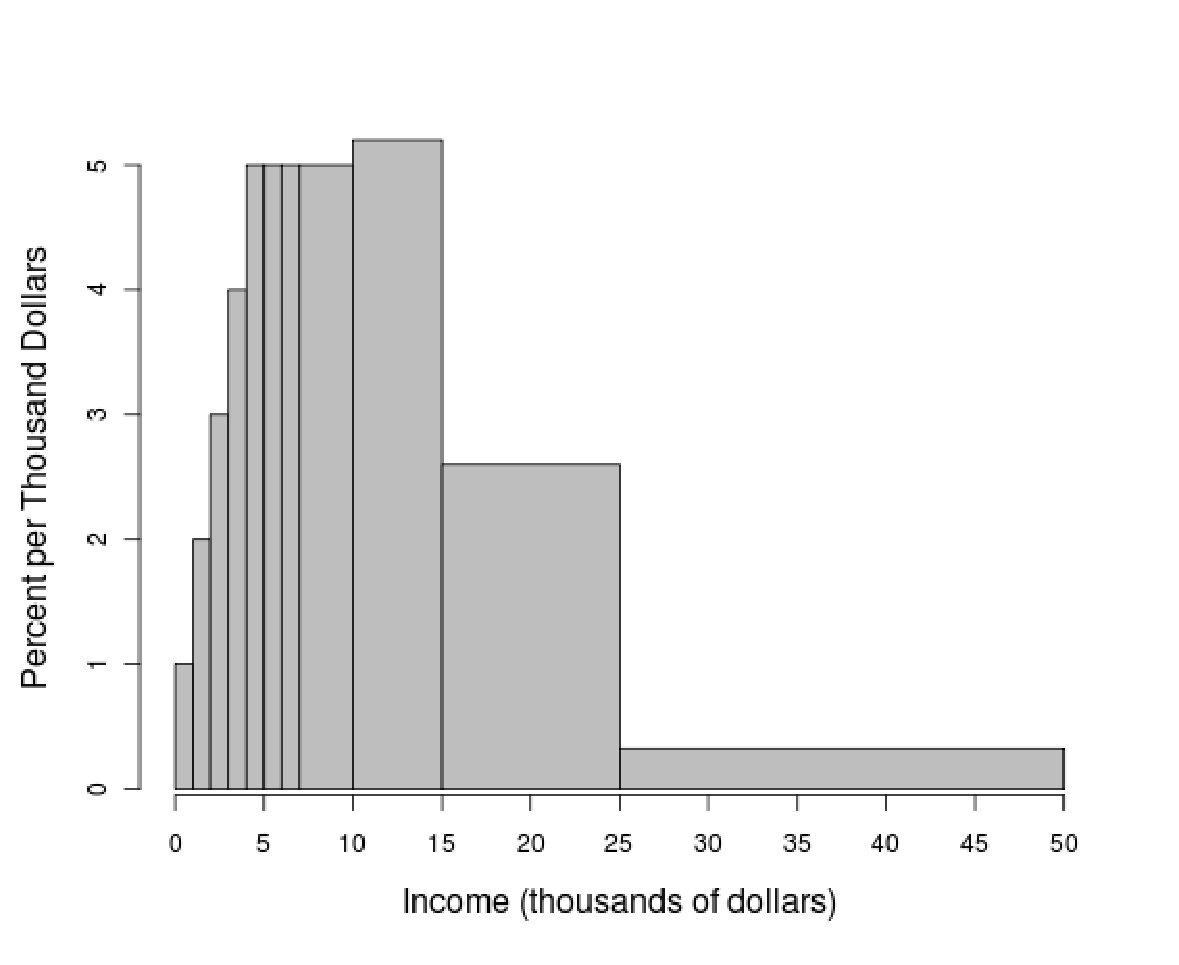
\includegraphics[height=1.8in]{Fig4p37.eps}}
\psframe[linewidth=0.02,linecolor=gray](-6.2,-7)(6.2,2.2)
\psframe[linewidth=0.02,linecolor=gray](-6.15,-6.95)(6.15,2.15)
\rput(0,1.4){\color{myblue}\large Math 207:  Statistics}
\rput(0,0.6){\color{myblue}The Histogram}
%\psframebox(0,0)(4,4)
\rput(0,-4.2){\scriptsize Dr.~Ralph Wojtowicz}
\rput(0,-4.7){\scriptsize Mathematics Department}
\rput(0,-5.5){
\includegraphics[height=1cm]{su-long.eps}}
\end{pspicture}
\end{center}

\end{frame}

%\section[Outline]{}

\addtocounter{page}{-1}
\addtocounter{framenumber}{-1}

{\footnotesize
\frame{\tableofcontents}
}

\section{Introduction}
\subsection{Descriptive Statistics}
\begin{frame}[t]\frametitle{Introduction}

{\small
\begin{itemize}
\item  \textbf{Graphical} tools (e.g., histograms
  and pie charts) can be used for summarizing and presenting data.
\item These show the manner in which the data values are distributed.
\item  \textbf{Numerical} tools (mean, standard deviation, median and percentiles) 
   are also used for describing data.
%\item Both chapters describe tools that involve a useful loss of information.
\end{itemize}
}

\begin{center}
{\footnotesize\begin{pspicture}(0,0)(3,4.4)
\psset{linewidth=0.02}
\rput(1.5,4){\rnode{Statistics}{\psframebox{Statistics}}}
\pnode(1.5,3){NULL}
\rput(0,3){\ovalnode{Descriptive}{\hspace{-8pt}\tiny\color{blue}
    \begin{tabular}{c}Descriptive\\ Statistics\end{tabular}\hspace{-8pt}}}
\rput(3,3){\ovalnode{Inferential}{\hspace{-8pt}\tiny\begin{tabular}{c}Inferential\\ Statistics\end{tabular}\hspace{-8pt}}}
\rput[t](0,2){\tiny\rnode{ID}{\psframebox{\hspace{-4pt}\begin{tabular}{l}Includes\\ 
        $\bullet$ Collecting\\ 
        $\bullet$ Organizing\\ 
        $\bullet$ \color{blue}Summarizing\\ 
        $\bullet$ \color{blue}Presenting\\ 
        {\color{blue}data}\end{tabular}\hspace{-4pt}}}}
\rput[t](3,2){\tiny\rnode{II}{\psframebox{\hspace{-4pt}\begin{tabular}{l}Includes\\ 
        $\bullet$ Making inferences\\ 
        $\bullet$ Hypothesis testing\\ 
        $\bullet$ Determining \\ \hphantom{$\bullet$} relationships\\ 
        $\bullet$ Making predictions\\ \end{tabular}\hspace{-4pt}}}}
\ncline{->}{Statistics}{NULL}
\ncline{->}{NULL}{Descriptive}
\ncline{->}{NULL}{Inferential}
\ncline{->}{Descriptive}{ID}
\ncline{->}{Inferential}{II}
\end{pspicture}}
\end{center}
\end{frame}

\subsection{Reading a Histogram}
\begin{frame}[t]\frametitle{Reading a Histogram}
{\ }\vspace{-20pt}

{\small
\begin{itemize}
\item A \textbf{histogram} is a graph used to summarize data.
\item The total area under the curve is 1 (that is, 100\%).
\item The horizontal axis is divided into \textbf{class intervals}.
\item The area of a rectangle is proportional to the percentage of data values in the class interval.\vspace{-20pt}
\end{itemize}

\begin{center}
{\setlength{\tabcolsep}{.2in}\begin{tabular}{cc}
\newcommand{\C}{\hphantom{\color{white},}}
\newcommand{\Z}{\hphantom{0}}
  \raisebox{1.0in}{\scriptsize\setlength{\tabcolsep}{2pt}
  \begin{tabular}{cc}
   Income Level & \hfill Percent\\[1pt]\hline
   \Z\Z\Z\C\Z\Z\$0--\$1,000\Z\Z & \Z1\vphantom{\large Y}\\
   \Z\$1,000--\$2,000\Z     & \Z2\\
   \Z\$2,000--\$3,000\Z     & \Z3\\
   \Z\$3,000--\$4,000\Z     & \Z4\\
   \Z\$4,000--\$5,000\Z     & \Z5\\
   \Z\$5,000--\$6,000\Z     & \Z5\\
   \Z\$6,000--\$7,000\Z     & \Z5\\
   \Z\$7,000--\$10,000      & 15\\
   \$10,000--\$15,000       & 26\\
   \$15,000--\$25,000       & 26\\
   \$25,000--\$50,000       & \Z8\\
   \$50,000 and over        & \Z1
  \end{tabular}}
&
  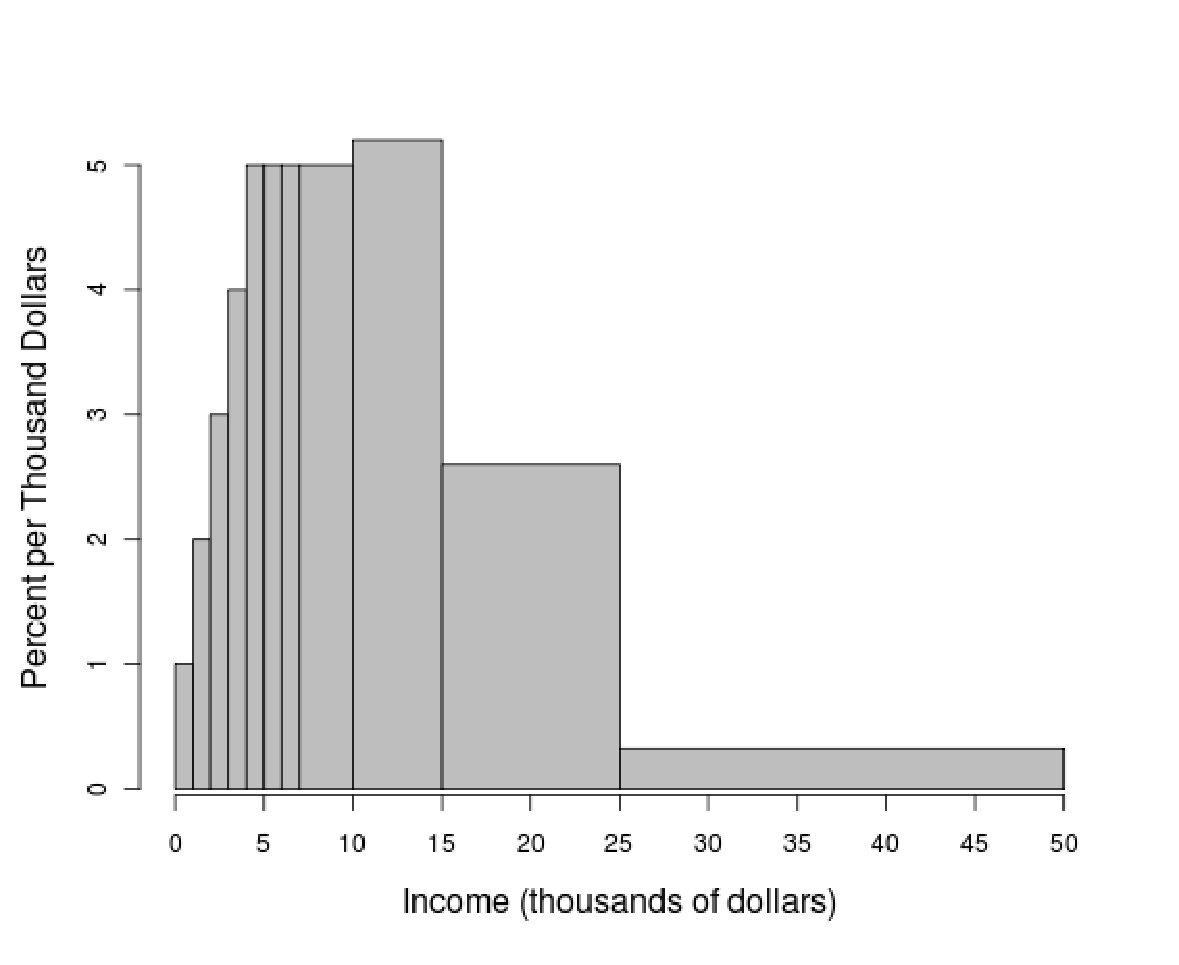
\includegraphics[height=2in, bb=0 0 550 400, clip]{Fig4p37.eps}
\rput[r](-1.5,4){\footnotesize 1973 data}
\end{tabular}}
\end{center}
}
\label{population}
\end{frame}


\section{Drawing a Histogram}

\subsection{Drawing a Histogram from a Distribution Table}
\begin{frame}[t]\frametitle{Drawing a Histogram from a Distribution Table}
{\ }\vspace{-20pt}

{\footnotesize
\begin{itemize}
\item A \textbf{\color{blue}distribution table} shows the percentage of data in each class interval. % (see Slide~\pageref{population}).
\item Choose an \textbf{endpoint convention} (e.g.,~put left endpoints in class intervals).
\item Use the class intervals to draw horizontal axis.
\item To figure out the height of a block over a class interval, divide the percentage by the length of the interval.\vspace{.075in}
\end{itemize}
}
%\begin{center}
{\setlength{\tabcolsep}{.2in}\begin{tabular}{ccc}
\newcommand{\C}{\hphantom{\color{white},}}
\newcommand{\Z}{\hphantom{0}}
  \rput(1.75,2.0){\scriptsize\setlength{\tabcolsep}{2pt}
  \begin{tabular}{cccc}
   \color{blue}Income Level & \hfill \color{blue} Percent & Width & Height\\[1pt]\hline
\color{blue}   \Z\Z\Z\C\Z\Z\$0--\$1,000\Z\Z & \color{blue}\Z1\vphantom{\large Y} & \Z1 & 1.0\\
\color{blue}   \Z\$1,000--\$2,000\Z     & \color{blue}\Z2 & \Z1 & 2.0\\
\color{blue}   \Z\$2,000--\$3,000\Z     & \color{blue}\Z3 & \Z1 & 3.0\\
\color{blue}   \Z\$3,000--\$4,000\Z     & \color{blue}\Z4 & \Z1 & 4.0\\
\color{blue}   \Z\$4,000--\$5,000\Z     & \color{blue}\Z5 & \Z1 & 5.0\\
\color{blue}   \Z\$5,000--\$6,000\Z     & \color{blue}\Z5 & \Z1 & 5.0\\
\color{blue}   \Z\$6,000--\$7,000\Z     & \color{blue}\Z5 & \Z1 & 5.0\\
\color{blue}   \Z\$7,000--\$10,000      & \color{blue}15 & \Z3 & 5.0\\
\color{blue}   \$10,000--\$15,000       & \color{blue}26 & \Z5 & 5.2\\
\color{blue}   \$15,000--\$25,000       & \color{blue}26 & 10 & 2.6\\
\color{blue}   \$25,000--\$50,000       & \color{blue}\Z8 & 25 & 0.3\\
\color{blue}   \$50,000 and over        & \color{blue}\Z1 
  \end{tabular}}
&\hspace{1.06in} & 
  \raisebox{-15pt}{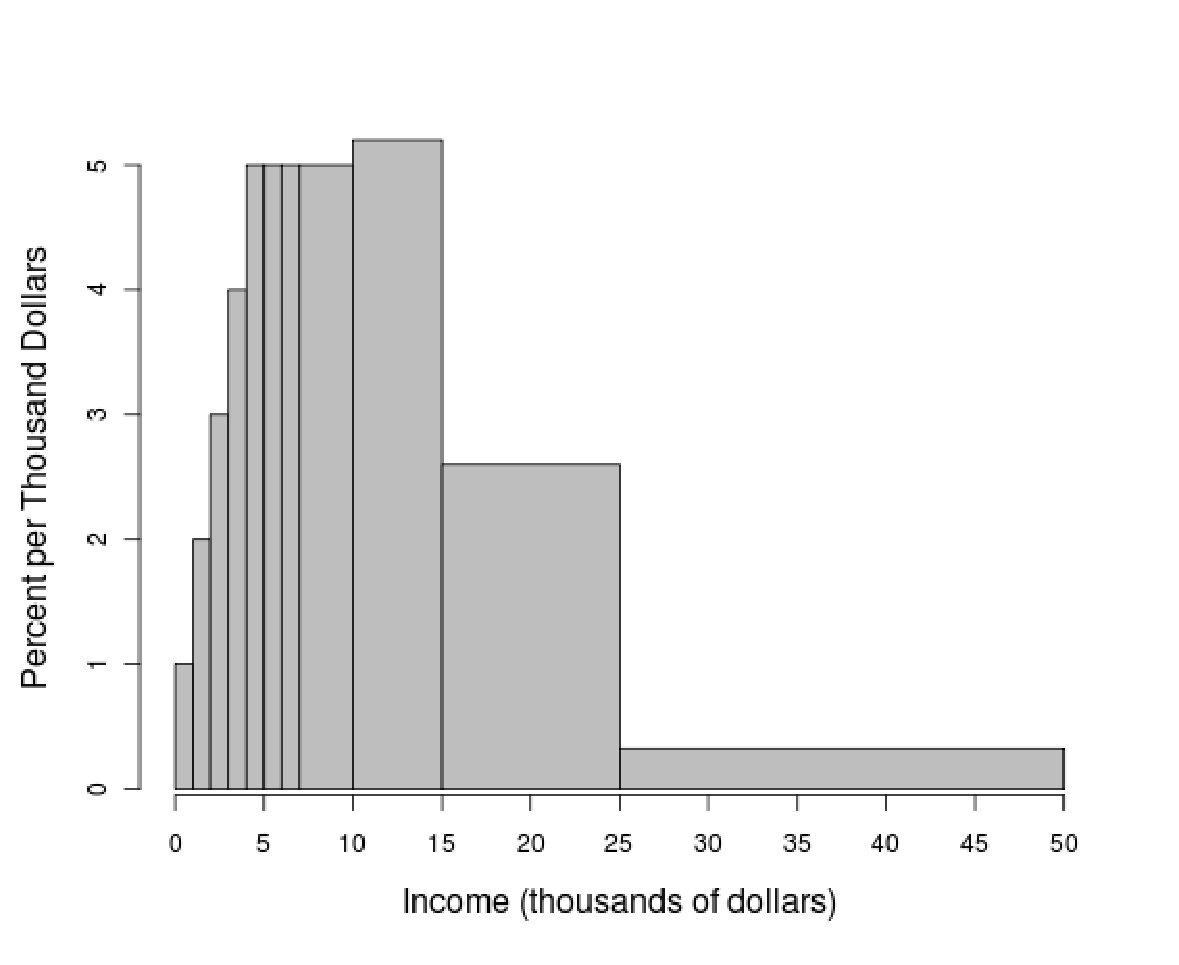
\includegraphics[height=2in, bb=0 0 550 400, clip]{Fig4p37.eps}}
\rput[r](-1.62,3.46){\footnotesize 1973 data}
\end{tabular}}
%\end{center}
\end{frame}


\subsection{Generating a Histogram from Data}
\begin{frame}[t]\frametitle{Generating a Histogram from Data}
{\ }\vspace{-20pt}

{\small
\begin{itemize}
\item Toss a fair coin $n=4$ times and count the number of heads.
\item Repeat this experiment $N=10$ times.
\item Example:  3, 1, 3, 2, 0, 2, 1, 4, 2, 0 heads in the 10 trials gives the histogram
below left.  
\item If we repeat the experiment $N=1000$ times, we get a histogram such as the one
shown below right.
\vspace{-.24in}

\end{itemize}
% For the first figure below, use the following.
% > xx <- CoinToss(10,4)
% [1] 3 1 3 2 0 2 1 4 2 0
% > hist(xx, prob=TRUE, breaks=seq(-0.5,4.5,by=1),xlab="Number of Heads", main="10 trials of 4 coin tosses")
% For the second figure, use this.
% > CoinTosshistogram(1000,4)
\begin{center}
\begin{tabular}{cc}
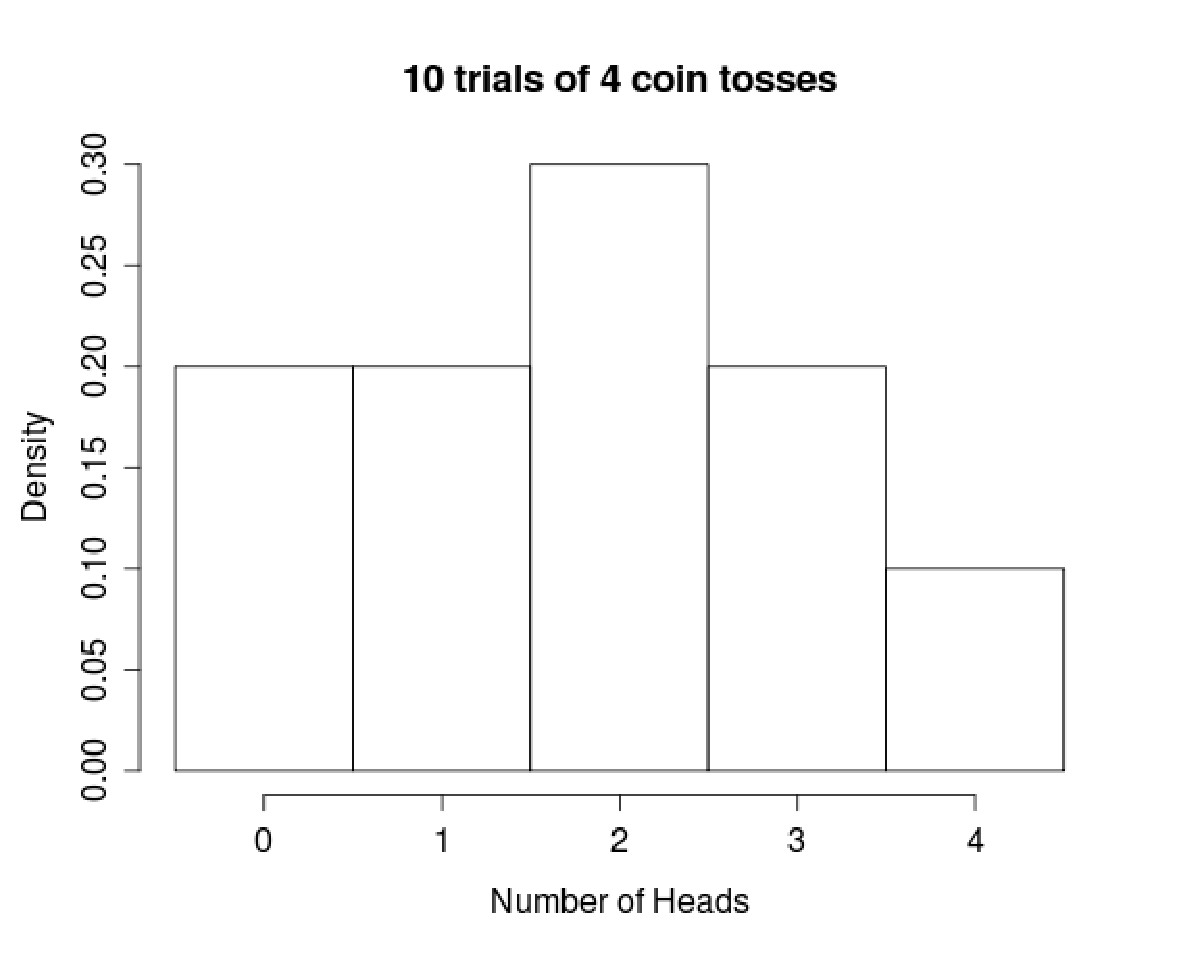
\includegraphics[height=1.8in]{CoinTrials.eps} &
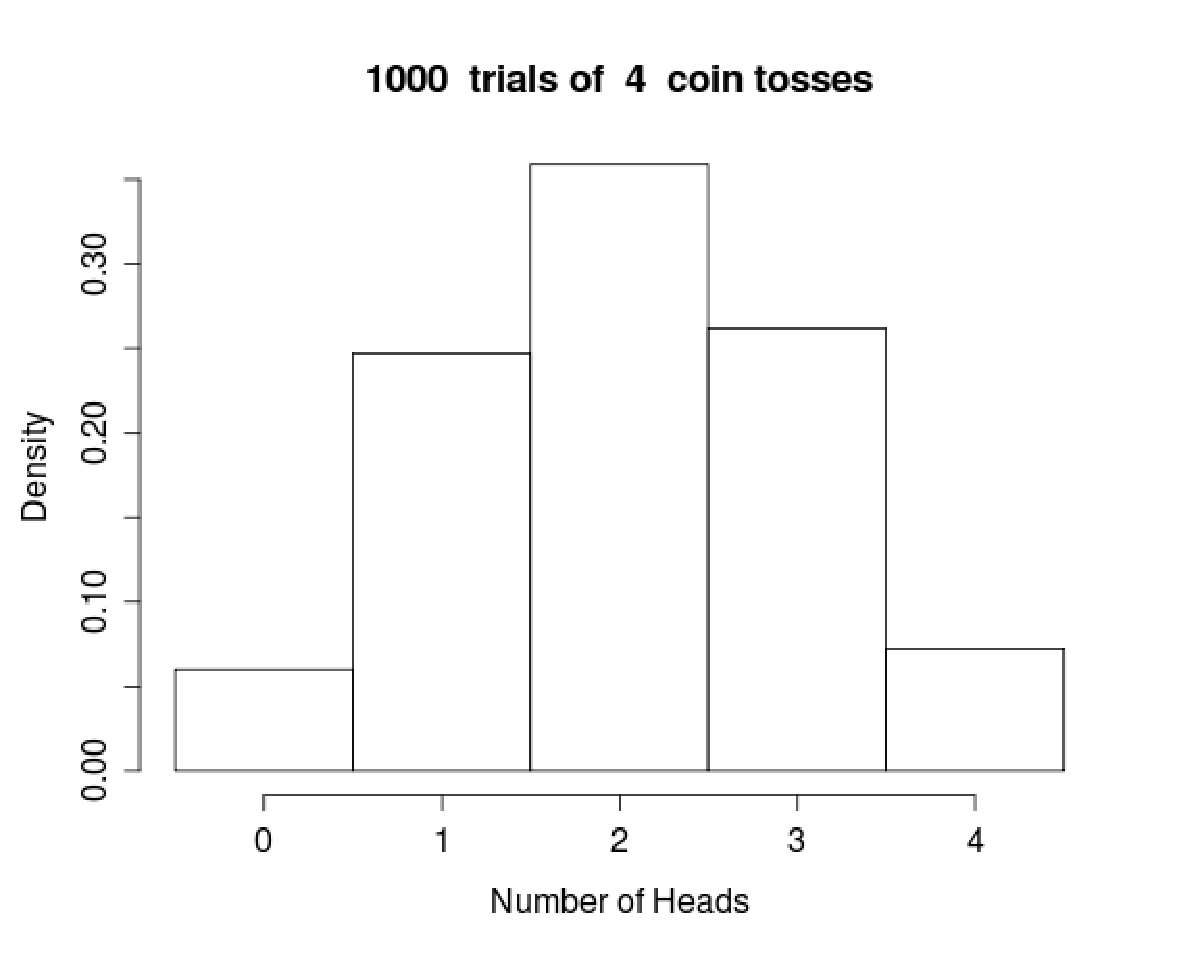
\includegraphics[height=1.8in]{CoinTrials2.eps}
\end{tabular}
\end{center}
}
\end{frame}


\begin{frame}[t]\frametitle{Generating a Histogram from Data (Example)}
{\ }\vspace{-20pt}
\scriptsize
\newcommand{\Z}{\hphantom{0}}
\begin{itemize}
\item Simulate rolling 20 dice:\\
\uncover<2->{\scriptsize\texttt{> sample(1:6, 20, replace=T)}}\\
\uncover<2->{\scriptsize\texttt{[1] 3 6 4 5 2 6 3 4 5 4 5 3 2 3 6 3 2 1 2 3}}
\item<3-> Create a distribution table:
\uncover<4->{\rput(4.5,-1.6){\scriptsize \begin{tabular}{ccc}
\scriptsize Number  & Number &         \\
\scriptsize of Dots & of Rolls & Percent\\\hline
1 &  1 & $\frac{1}{20} = 0.05 = \Z5\%$\vphantom{\LARGE Y}\\[3.5pt]
2 &  4 & $\frac{4}{20} = 0.20 = 20\%$\\[3.5pt]
3 &  6 & $\frac{6}{20} = 0.05 = 30\%$\\[3.5pt]
4 &  3 & $\frac{3}{20} = 0.05 = 15\%$\\[3.5pt]
5 &  3 & $\frac{3}{20} = 0.05 = 15\%$\\[3.5pt]
6 &  3 & $\frac{3}{20} = 0.05 = 15\%$\\
\end{tabular}}}\vspace{0.4in}
\item<5-> Draw the histogram (called a bar plot\\ since the variable isn't continuous):
\uncover<6->{\begin{center}
\begin{pspicture}(3,0)(6,3.3)
\psset{yunit=0.1}
\psframe*[linecolor=blue](0,0)(1,5)
\psframe*[linecolor=blue](1,0)(2,20)
\psframe*[linecolor=blue](2,0)(3,30)
\psframe*[linecolor=blue](3,0)(4,15)
\psframe*[linecolor=blue](4,0)(5,15)
\psframe*[linecolor=blue](5,0)(6,15)
\psline[linewidth=0.02](0,0)(0,30)
\rput[r](-0.3,5){5}   \psline[linewidth=0.02](0,5)(-0.2,5)
\rput[r](-0.3,10){10} \psline[linewidth=0.02](0,10)(-0.2,10)
\rput[r](-0.3,15){15} \psline[linewidth=0.02](0,15)(-0.2,15)
\rput[r](-0.3,20){20} \psline[linewidth=0.02](0,20)(-0.2,20)
\rput[r](-0.3,25){25} \psline[linewidth=0.02](0,25)(-0.2,25)
\rput[r](-0.3,30){30} \psline[linewidth=0.02](0,30)(-0.2,30)
\rput(0.5,-2){1}
\rput(1.5,-2){2}
\rput(2.5,-2){3}
\rput(3.5,-2){4}
\rput(4.5,-2){5}
\rput(5.5,-2){6}
\rput(3,-5.5){Number of Dots}
\rput{90}(-1,15){Percent of Rolls}
\end{pspicture}
\end{center}}
\end{itemize}


\end{frame}

\section{The Density Scale}
\subsection{The Density Scale}
\begin{frame}[t]\frametitle{The Density Scale}
{\ }\vspace{-30pt}

%{\ }\vspace{-.22in}
%> edu <- c(2,4,4,11,39,18,21)
%> eduI <- c(5,3,1,3,1,3,1)
%> barplot(edu/eduI, eduI, space=0, xlab="Educational Level (Years)", ylab="Percent Per Year", cex.axis=0.75)
%> axis(1, seq(0,18, by=2), cex.axis=0.75)
{\small%
\begin{pspicture}(0,0)(0,0)%
\rput(8.8,-5.08){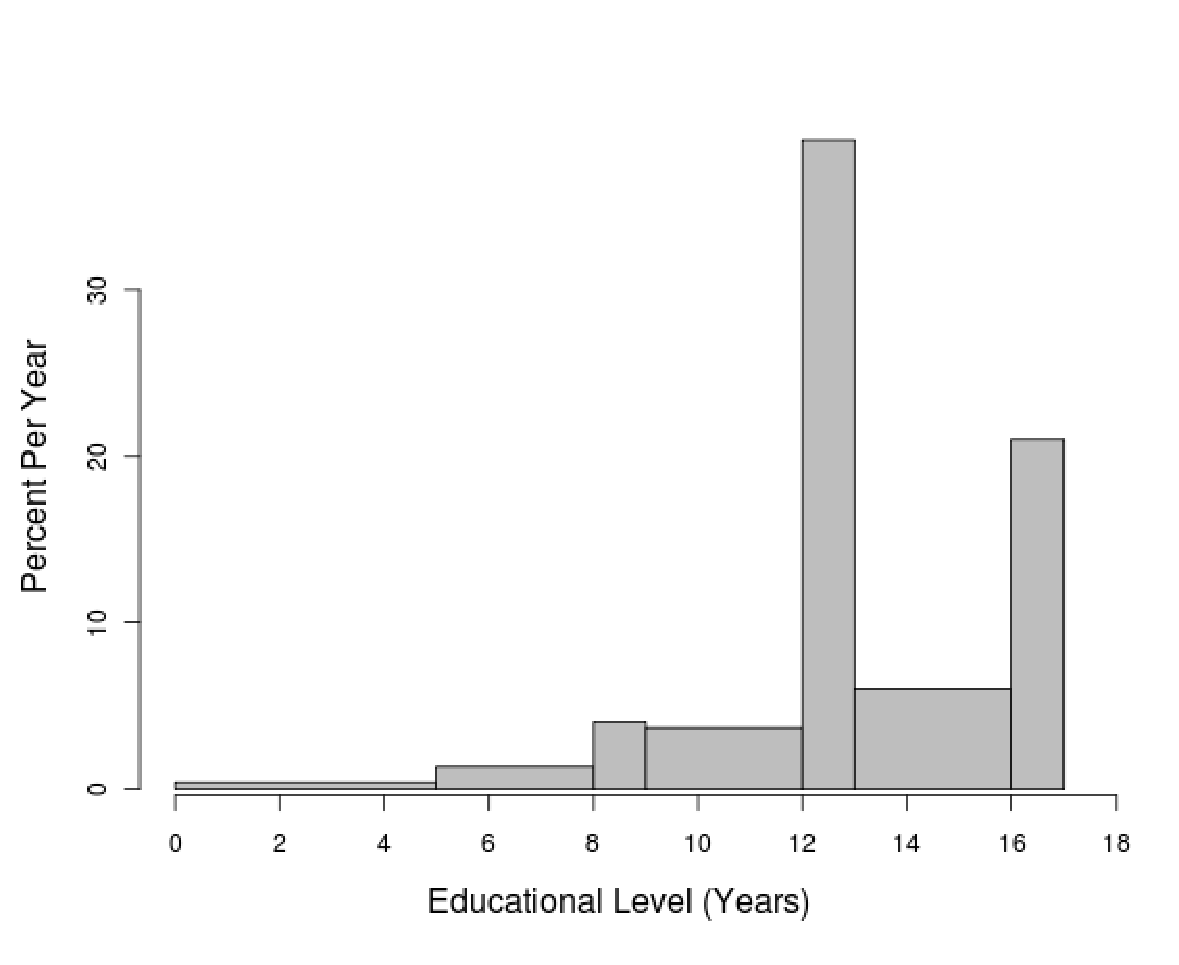
\includegraphics[height=2in, bb=0 0 550 407, clip]{Fig5p39.eps}}
\end{pspicture}%
\begin{itemize}
\item The histogram below shows years of school completed by persons age 25 and older in the U.S. in 1991.
\item Endpoint convention: years of school \textit{completed} 
  (e.g.,~people who dropped out part way through ninth grade are in the 8--9 block)
\item Units on the vertical axis are percent (of people) per year (of schooling).
\item Area represents percent. Total area $=$ 100\%.
\item Box heights show \textit{crowding}.
\item Peaks: 8--9, 12--13 and 16--17\vspace{-3pt}
\end{itemize}

{{\ }\hspace{22pt}
\footnotesize\begin{tabular}{cc}
Years & Percent\\[1pt]\hline
0--5 & 2\vphantom{\large{Y}}\\
5--8 & 4\\
8--9 & 4\\
9--12 & 11\\
12--13 & 39\\
13--16 & 18\\
16 or more & 21
\end{tabular}}
}
%\label{lastpage}
\end{frame}

\section[Variables]{Variables}
\subsection{Variables}
\begin{frame}[t]\frametitle{Variables}
{\footnotesize
\begin{itemize}
\item A (random) \textbf{variable} is a measurement that depends on the outcome of a (random) event.
\item \footnotesize\textbf{Quantitative} variables have numeric values.  
  \begin{itemize} 
     \item \footnotesize\textbf{Continuous} variables can assume a continuum of values:  
        Examples include 
      income, temperature, pressure, mass, and speed. 
     \item \footnotesize
        A \textbf{discrete} variable can assume only finitely (or countably) many values.
       Examples include: family size, and number of engine cylinders.
  \end{itemize}
\item \footnotesize
   \textbf{Qualitative} variables are non-numeric.  
   \begin{itemize}
   \item \footnotesize They can be \textbf{Ordered}:  good, better, best; or 
    sometimes, always, never
   \item \footnotesize or they can be \textbf{Unordered} such as eye color, marital status
     or automobile transmission type
   \end{itemize}
\end{itemize}}


\begin{center}
{\footnotesize\begin{pspicture}(-1.5,0)(7.5,1.8)
\psset{linewidth=0.02, nodesep=2pt, xunit=3,yunit=0.9}
\rput(1,2){\rnode{Variables}{Variables}}
\rput(0,1){\rnode{Qualitative}{Qualitative}}
\rput(2,1){\rnode{Quantitative}{Quantitative}}
\rput(1.5,0){\rnode{Discrete}{Discrete}}
\rput(2.5,0){\rnode{Continuous}{Continuous}}
\rput(-0.5,0){\rnode{Ordered}{Ordered}}
\rput(0.5,0){\rnode{Unordered}{Unordered}}
\ncline{Variables}{Qualitative}
\ncline{Variables}{Quantitative}
\ncline{Quantitative}{Discrete}
\ncline{Quantitative}{Continuous}
\ncline{Qualitative}{Ordered}
\ncline{Qualitative}{Unordered}
\end{pspicture}}
\end{center}

\label{lastpage}
\end{frame}

\end{document}

\section[Controlling]{Controlling for a Variable}
\subsection{Controlling for a Variable}
\begin{frame}[t]\frametitle{Controlling for a Variable}

{\small
\begin{itemize}
\item Observational studies: subjects assign themselves to treatment and control
\item Association between treatment and outcome is circumstantial evidence for causation
  in such studies.
\item Technique:  compare small, more homogeneous groups (e.g.,~age, gender)
\end{itemize}}

% users <- c(0.4, 1.0, 2.0, 3.0, 3.5, 2.6, 2.5, 2.0, 1.0, 0.6, 0.2)
% userClassWidths <- c(10,5,5,5,5,5,5,5,5,10,10)
% sum(users*userClassWidths)
% nonUsers <- c(0.6, 2.2, 3.5, 3.6, 2.1, 1.8, 1.4, 0.8, 0.5, 0.1)
% nonUserClassWidths <- c(10,10,5,5,5,5,5,5,10,10)
% sum(nonUsers*nonUserClassWidths)
\end{frame}



\end{document}

\subsection{Drawing a Histogram from Data}
\begin{frame}[t]\frametitle{Drawing a Histogram from Data}
text
\end{frame}



\section[Variables]{Variables}
\subsection{Variables}
\begin{frame}[t]\frametitle{Variables}
{\small
\begin{itemize}
\item A (random) \textbf{variable} is a measurement that depends on the outcome of a (random) event.
\item \textbf{Quantitative} variables have numeric values.  
  \begin{itemize} 
     \item \textbf{Continuous} variables can assume a continuum of values:  Examples include temperature, pressure, mass, and speed. 
     \item A \textbf{discrete} variable can assume only finitely (or countably) many values.
       Examples include: family size, and number of engine cylinders.
  \end{itemize}
\item \textbf{Qualitative} variables are non-numeric.  Values are typically  descriptive words or phrases.
 Examples include:  marriage status, true or false, employment status,  eye color, automobile transmission type.
\end{itemize}}

\begin{center}
{\footnotesize\begin{pspicture}(0,0)(3,2.2)
\psset{linewidth=0.02, nodesep=2pt}
\rput(1,2){\rnode{Variables}{Variables}}
\rput(0,1){\rnode{Qualitative}{Qualitative}}
\rput(2,1){\rnode{Quantitative}{Quantitative}}
\rput(1,0){\rnode{Discrete}{Discrete}}
\rput(3,0){\rnode{Continuous}{Continuous}}
\ncline{Variables}{Qualitative}
\ncline{Variables}{Quantitative}
\ncline{Quantitative}{Discrete}
\ncline{Quantitative}{Continuous}
\end{pspicture}}
\end{center}
\end{frame}



\end{document} 


\begin{frame}[t]\frametitle{A Histogram with Class Labels}
text
\end{frame}



\section{Cross-Tabulation}
\subsection{Cross-Tabulation}
\begin{frame}[t]\frametitle{Cross-Tabulation}

\end{frame}

\section{Selective Breeding}
\subsection{Selective Breeding}
\begin{frame}[t]\frametitle{Selective Breeding}

\label{lastpage}
\end{frame}



\end{document}
